\section{Method}
\label{sec:method}
We present a novel inverse rendering framework for reconstructing reflective objects from multi-view RGB images under unknown illumination. As illustrated in Fig.~\ref{fig:pipline}, our approach decomposes the problem into two sequential stages: First, geometry reconstruction leverages deferred Gaussian splatting with split-sum approximation for efficient physically-based rendering while incorporating geometric priors from foundation models to mitigate geometry ambiguities (Sec.~\ref{sec:method-geo}). Second, with object geometry fixed, we refine material properties through Monte Carlo importance sampling of the full rendering equation to optimize BRDF parameters, enhanced by a spherical mipmap-based specular compensation mechanism for complex specular effects (Sec.~\ref{sec:method-ir}).
\subsection{Stage I: Geometry reconstruction}
\label{sec:method-geo}
\noindent\textbf{Split-sum Approximation.}
Within deferred shading using aggregated per-pixel material attributes, we compute the specular term via split-sum approximation~\cite{munkberg2022extracting} to mitigate its computational cost. This decomposes the rendering integral into:
\begin{equation}
\label{eq:split_sum}
L_s(\boldsymbol{\omega}_o) \approx \underbrace{\int_{\Omega} f_s(\cdot) (\boldsymbol{\omega}_i\!\cdot\!\boldsymbol{n}) d\boldsymbol{\omega}_i}_{\text{BRDF factor}} \cdot \underbrace{\int_{\Omega} L_i(\cdot) D(\cdot)(\boldsymbol{\omega}_i\!\cdot\!\boldsymbol{n})  d\boldsymbol{\omega}_i}_{\text{Lighting factor}}.
\end{equation}
The BRDF factor, dependent on material roughness $R$ and normal angle $(\boldsymbol{\omega}_i \cdot \boldsymbol{n})$, is precomputed into a 2D lookup texture. The lighting factor integrates environmental radiance over the specular lobe using trilinear interpolation in pre-filtered Mipmap cubemaps, indexed by reflected direction $\boldsymbol{\omega}_r = 2(\boldsymbol{n} \cdot \boldsymbol{\omega}_o)\boldsymbol{n} - \boldsymbol{\omega}_o$ and roughness $R$. 
While computationally efficient, this approximation inherently limits high-frequency specular modeling, particularly on low-roughness surfaces, necessitating refinement with the full rendering equation.

\noindent\textbf{Supervision from Foundation Models.}
To mitigate geometry ambiguities in specular surface reconstruction, we leverage robust geometric priors from large-scale vision foundation models~\cite{Ke_Obukhov_Huang_Metzger_Daudt_Schindler_2023, garcia2025fine}. These models generate monocular depth $\tilde{D}$ and normal $\tilde{N}$ estimates invariant to view-dependent effects, providing reliable supervision even for highly reflective surfaces where multi-view consistency fails.

We incorporate these priors as regularization during Gaussian optimization. The predicted normals $\tilde{N}$ supervise rendered normals $\hat{N}$ via a dual loss:
\begin{equation}
\label{eq:L-geo-n}
\mathcal{L}_{\text{geo-n}} = \|\hat{N} - \tilde{N}\|_1 + \lambda \left(1 - \frac{\hat{N} \cdot \tilde{N}}{\|\hat{N}\| \|\tilde{N}\|}\right),
\end{equation}
where $\lambda$ balances magnitude and angular alignment. For depth supervision, we employ a scale-invariant formulation~\cite{ranftl2020towards} with predicted normals $\tilde{D}$ and rendered normals $\hat{D}$:
\begin{equation}
\label{eq:L-geo-d}
\mathcal{L}_{\text{geo-d}} = \min_{\omega, b} \sum_{p} \left[ (\omega \hat{D} + b) - \tilde{D} \right]^2,
\end{equation}
with $\omega$ and $b$ optimized per-view via least squares. As demonstrated in Fig.~\ref{fig:normal_compa}, this geometric regularization explicitly enhances curvature continuity while suppressing surface noise from specular interference.

\noindent\textbf{Training Loss.}
The complete training objective integrates physical rendering losses with our geometric priors:
\begin{equation}
\begin{split}
\mathcal{L}^1 = & \mathcal{L}_{\mathrm{c}} 
+ \lambda_{\mathrm{n}} \mathcal{L}_{\mathrm{n}} 
+ \lambda_{\mathrm{o}} \mathcal{L}_{\mathrm{o}} 
+ \lambda_{\text{smooth}} \mathcal{L}_{\text{smooth}} \\
& + \lambda_{\text{geo-n}} \mathcal{L}_{\text{geo-n}} 
+ \lambda_{\text{geo-d}} \mathcal{L}_{\text{geo-d}}.
\end{split}
\end{equation}
Following 2DGS~\cite{huang20242dgs}, we utilize its core components including the RGB reconstruction loss $\mathcal{L}_\mathrm{c} = \|c_{\text{render}} - C_{gt}\|_1$ and the normal alignment loss defined as $\mathcal{L}_\mathrm{n} = 1 - \tilde{\boldsymbol{N}}^{\mathrm{T}} \boldsymbol{N}$.
$\mathcal{L}_\mathrm{o}$ is a binary cross-entropy loss constraining the geometry using the provided object mask $\mathcal{M}$ defined as $\mathcal{L}_{\mathrm{o}}=-\mathcal{M} \log \mathcal{O}-(1-\mathcal{M}) \log (1-\mathcal{O})$, where $\mathcal{O}=\sum_{i=1}^N T_i \alpha_i$ denotes the accumulated opacity map. 
To provide joint regularization for both normals and depth, we incorporate an edge-aware smoothness term 
$\mathcal{L}_\text{smooth} = \|\nabla \boldsymbol{N}\| \exp\left(-\|\nabla C_{gt}\|\right)$.
Finally, our novel geometric regularizers $\mathcal{L}_\text{geo-n}$ and $\mathcal{L}_\text{geo-d}$, 
defined in Eq.~\ref{eq:L-geo-n} and Eq.~\ref{eq:L-geo-d}, enforce alignment with foundation model priors.
\begin{figure}[h!]
    \vspace{-1em}
    \centering
    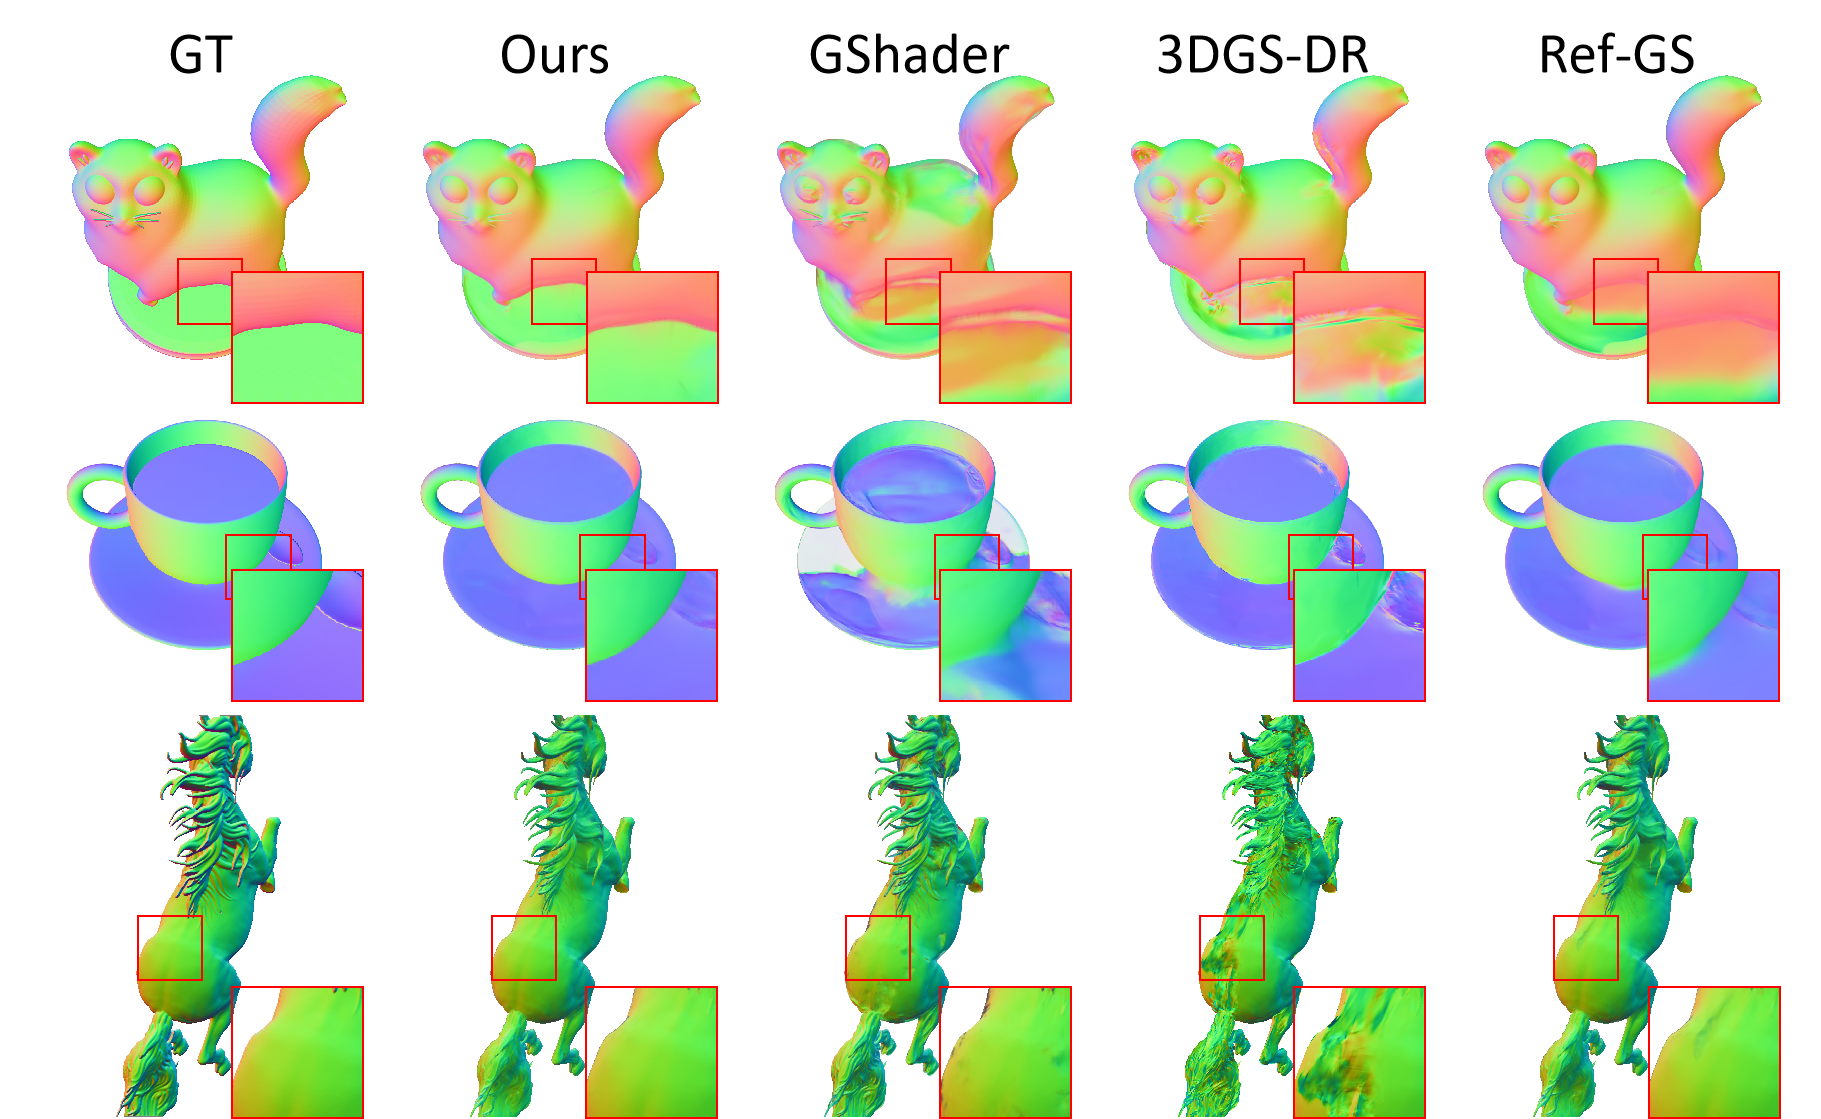
\includegraphics[width=1\linewidth]{res/normal_compa.png}
    \caption{Per-scene qualitative comparisons of normals.}
    \label{fig:normal_compa}
    \vspace{-1em}
\end{figure}

% Please add the following required packages to your document preamble:
% \usepackage{graphicx}
% \usepackage[table,xcdraw]{xcolor}
% Beamer presentation requires \usepackage{colortbl} instead of \usepackage[table,xcdraw]{xcolor}
\begin{table*}[h!]
\vspace{-1em}
\centering
\captionsetup{width=0.9\textwidth}
\caption{Quantitative comparison of average novel view synthesis metrics on synthesized test views.
Deeper red indicates better performance.
Ours(geo) corresponds to results from our first-stage geometric reconstruction (Sec.~\ref{sec:method-geo}), while Ours(ir) corresponds to those from our second-stage inverse rendering (Sec.~\ref{sec:method-ir}).}
\label{tab:quality_compa}
\resizebox{0.95\textwidth}{!}{%
\begin{tabular}{l|ccc|ccc|ccc}
\hline
\hline
\textbf{Datasets} & \multicolumn{3}{c|}{\textbf{Shiny Synthetic\cite{verbin2022refnerf}}}                                                 & \multicolumn{3}{c|}{\textbf{Glossy Synthetic\cite{liu2023nero}}}                                                & \multicolumn{3}{c}{\textbf{Shiny Real\cite{verbin2022refnerf}}}                                                       \\ \hline
                  & PSNR ↑                        & SSIM ↑                        & LPIPS ↓                       & PSNR ↑                        & SSIM ↑                        & LPIPS ↓                       & PSNR ↑                        & SSIM ↑                        & LPIPS ↓                       \\ \hline
Ref-NeRF\cite{verbin2022refnerf}          & 33.13                         & 0.961                         & 0.080                         & 25.65                         & 0.905                         & 0.112                         & 23.62                         & 0.646                         & 0.239                         \\
ENVIDR\cite{liang2023envidr}            & 33.46                         & \cellcolor[HTML]{FD6864}0.979 & \cellcolor[HTML]{FD6864}0.046 & 29.06                         & 0.947                         & 0.060                         & 23.00                         & 0.606                         & 0.332                         \\
2DGS\cite{huang20242dgs}              & 29.58                         & 0.946                         & 0.084                         & 26.07                         & 0.918                         & 0.088                         & 24.15                         & 0.661                         & 0.292                         \\
GShader\cite{jiang2024gaussianshader}           & 31.97                         & 0.958                         & 0.067                         & 27.11                         & 0.922                         & 0.145                         & 23.46                         & 0.647                         & 0.257                         \\
R3DG\cite{gao2024r3dg}              & 27.77                         & 0.926                         & 0.112                         & 24.13                         & 0.892                         & 0.106                         & 21.98                         & 0.619                         & 0.349                         \\
3DGS-DR\cite{ye20243dgsdr}      & 34.00                         & 0.972                         & 0.059                         & 28.73                         & 0.948                         & 0.058                         & 24.37                         & 0.678                         & \cellcolor[HTML]{FFCCC9}0.232 \\
Ref-Gaussian\cite{yao2024refgaussian}            & \cellcolor[HTML]{FFCCC9}34.66 & 0.972                         & 0.055                         & \cellcolor[HTML]{FFCCC9}30.77 & \cellcolor[HTML]{FFCCC9}0.962 & \cellcolor[HTML]{FD6864}0.045 & \cellcolor[HTML]{FFCCC9}24.71 & \cellcolor[HTML]{FFCCC9}0.691 & 0.263                         \\
IRGS\cite{gu2025irgs}              & 28.39                         & 0.932                         & 0.110                         & 24.40                         & 0.892                         & 0.109                         & 21.38                         & 0.425                         & 0.486                         \\
Ours(geo)          & \cellcolor[HTML]{FD6864}35.03 & \cellcolor[HTML]{FFCCC9}0.975 & \cellcolor[HTML]{FFCCC9}0.055 & \cellcolor[HTML]{FD6864}30.83 & \cellcolor[HTML]{FD6864}0.962 & \cellcolor[HTML]{FFCCC9}0.048 & \cellcolor[HTML]{FD6864}26.56 & \cellcolor[HTML]{FD6864}0.783 & \cellcolor[HTML]{FD6864}0.178 \\
Ours(ir)          & 32.21                         & 0.959                         & 0.078                         & 29.38                         & 0.947                         & 0.060                         & 24.47                         & 0.687                         & 0.299                         \\ \hline
\hline
\end{tabular}%
}
\end{table*}

\subsection{Stage II: Inverse Rendering}
\label{sec:method-ir}
Building upon the reconstructed geometry from Stage I~\ref{sec:method-geo}, we now refine the initial BRDF estimation through physically accurate inverse rendering. This stage employs the full rendering equation to precisely optimize material parameters, including metalness $m$, albedo $a$, and roughness $\rho$, while leveraging Monte Carlo importance sampling for efficient incident radiance computation and rendering equation evaluation.

\noindent\textbf{Sampling Strategy.} 
We implement two physically-based importance sampling strategies for optimal variance reduction. For the diffuse component, we follow the Lambertian distribution with sampling probability:
\begin{equation}
p_d(\omega_i) = \frac{\cos\theta}{\pi},
\end{equation}
while for the specular component, we employ GGX normal distribution-based sampling~\cite{cook1982reflectance}:
\begin{equation}
p_s(\omega_i) = \frac{D(\boldsymbol{h}) \cos\theta}{4(\boldsymbol{\omega_o} \cdot \boldsymbol{h})}.
\end{equation}
To minimize variance in transitional regions between diffuse and specular responses, we integrate both sampling strategies through a balance heuristic~\cite{veach1998robust}. Defining strategy proportions $\pi_d = N_d / (N_d + N_s)$ and $\pi_s = N_s / (N_d + N_s)$, the weight for a sample $\omega_i$ from strategy $k \in \{d, s\}$ is computed as:
\begin{equation}
w_k(\omega_i) = \frac{\pi_k p_k(\omega_i)}{\sum_{m \in \{d,s\}} \pi_m p_m(\omega_i)}.
\end{equation}
The final radiance $L_o^{\mathrm{phys}}$ estimate combines both contributions:
\begin{align}
L_o^{\mathrm{diffuse}} &= \frac{1}{N_d} \sum_{i=1}^{N_d} \frac{f_d L_i (\boldsymbol{n} \cdot \omega_i) w_d}{p_d}, \\
L_o^{\mathrm{specular}} &= \frac{1}{N_s} \sum_{j=1}^{N_s} \frac{f_s L_j (\boldsymbol{n} \cdot \omega_j) w_s}{p_s}, \\
L_o^{\mathrm{pbr}} &= L_o^{\mathrm{diffuse}} + L_o^{\mathrm{specular}}.
\end{align}
This formulation adaptively balances sample contributions based on local material properties, significantly reducing noise while maintaining physical accuracy.

{
\setlength{\parindent}{0pt}
\textbf{Light parametrization.} The incident radiance $L_{\mathrm{i}}(\boldsymbol{\omega}_i, \boldsymbol{x})$ at surface point $\boldsymbol{x}$ along direction $\boldsymbol{\omega}_i$ (Eq.~\ref{eq:renderingEquation}) decomposes into direct radiance from distant sources and indirect radiance from scene surfaces:
\begin{equation}
L_{\mathrm{i}}\left(\boldsymbol{\omega}_i, \boldsymbol{x}\right)=V\left(\boldsymbol{\omega}_i, \boldsymbol{x}\right) L_{\mathrm{dir}}\left(\boldsymbol{\omega}_i\right)+L_{\mathrm{ind}}\left(\boldsymbol{\omega}_i, \boldsymbol{x}\right), 
\end{equation}
where direct radiance $L_{\mathrm{dir}}$ is parameterized via an environment cubemap, while visibility $V$ and indirect radiance $L_{\mathrm{ind}}$ are computed through IRGS's differentiable 2D Gaussian ray tracing~\cite{gu2025irgs}.
}
\begin{figure*}[h!]
    \vspace{-1em}
    \centering
    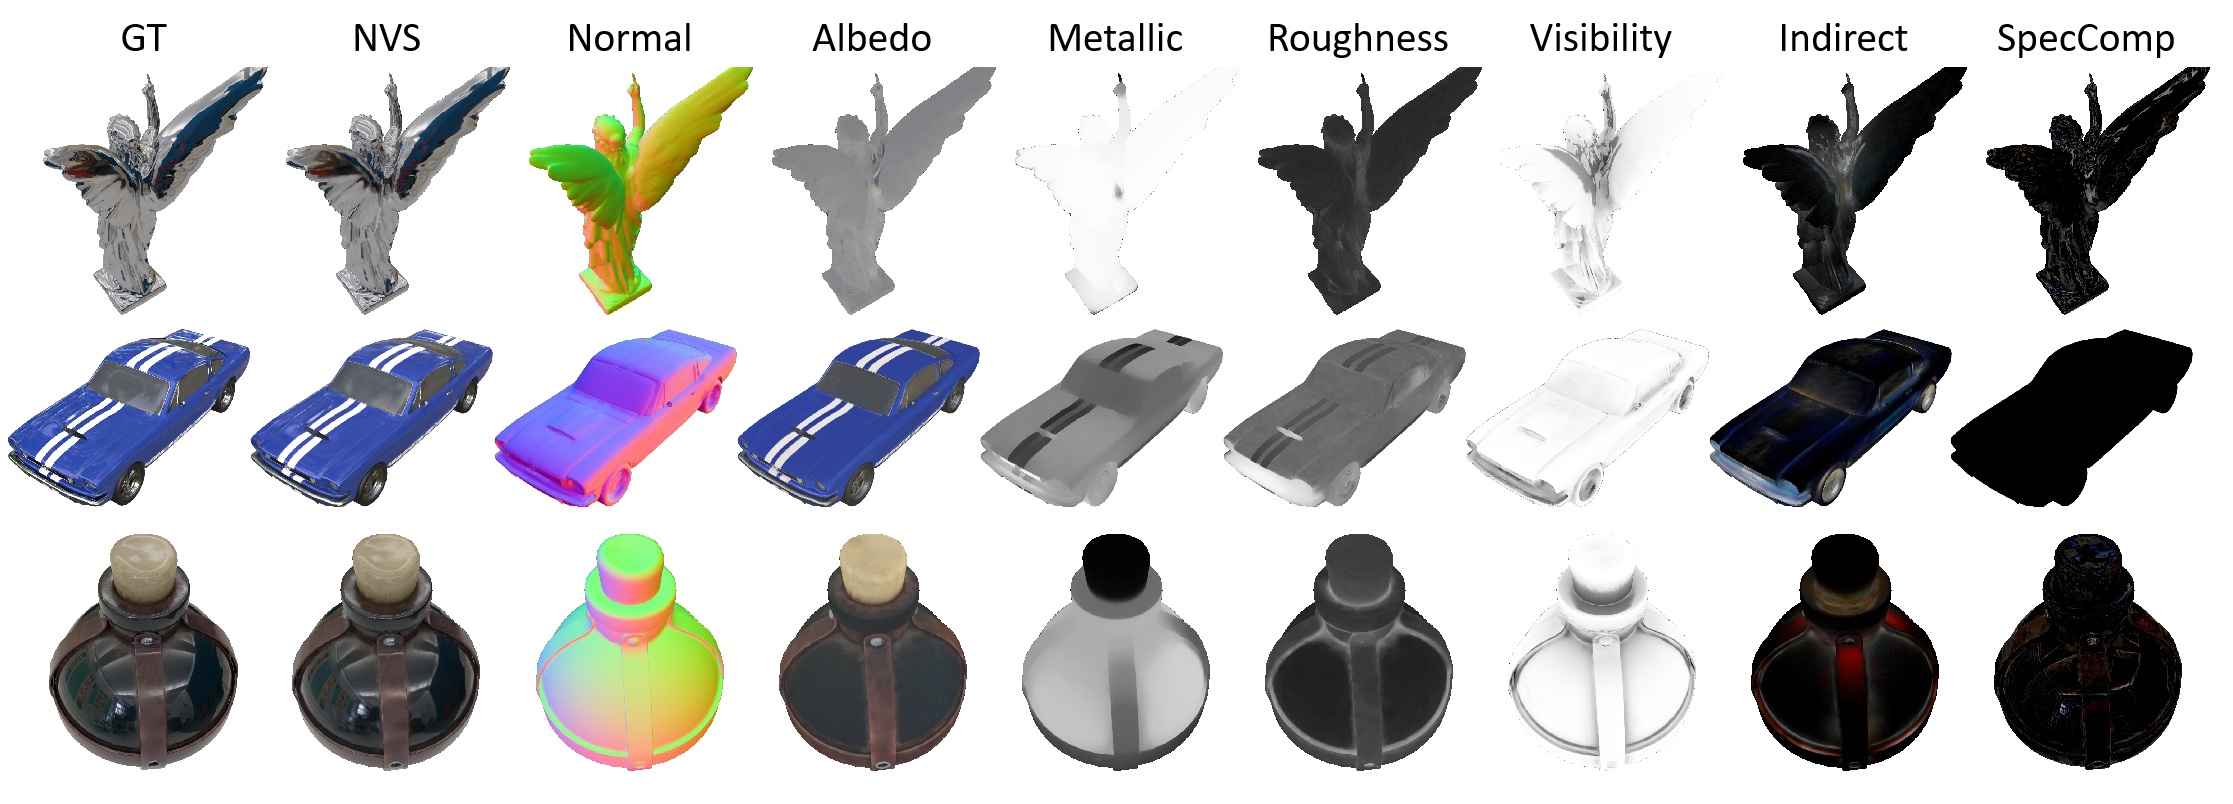
\includegraphics[width=0.9\linewidth]{res/results.png}
    \captionsetup{width=0.9\linewidth}
    \caption{Qualitative decomposition results of our model.}
    \label{fig:results}
    \vspace{-1em}
\end{figure*}

\begin{figure}
    \centering
    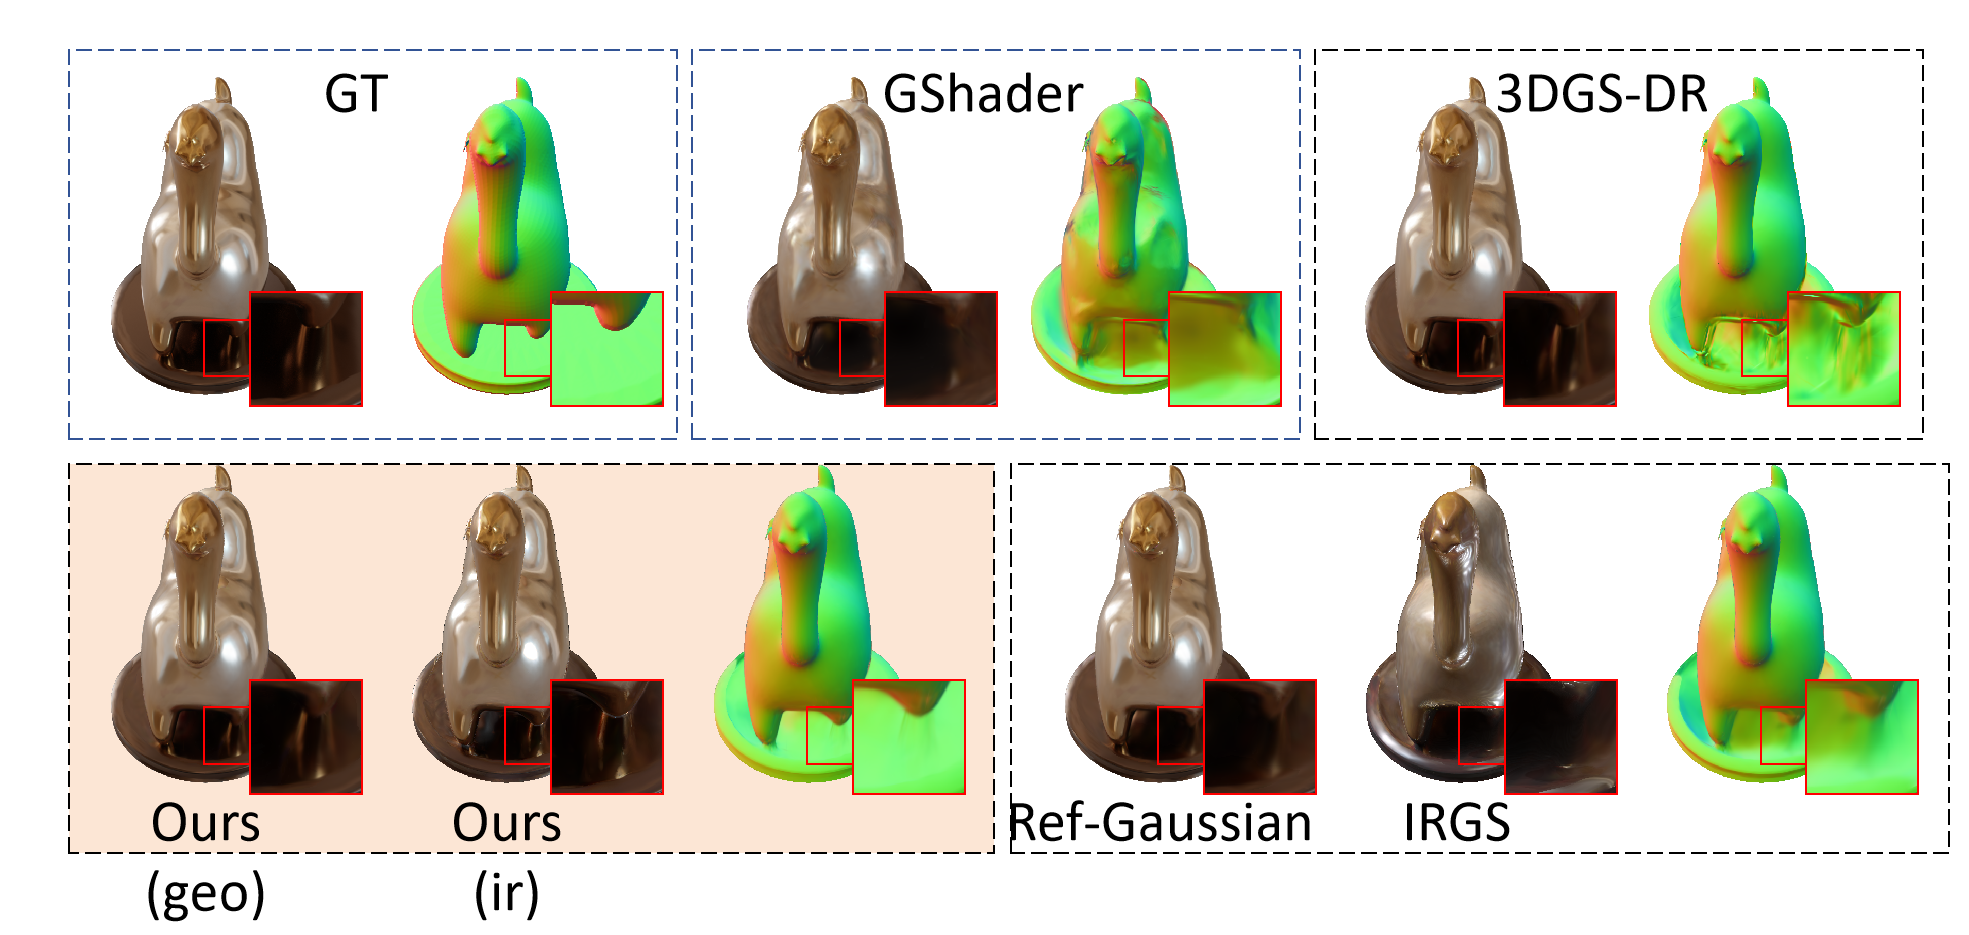
\includegraphics[width=1\linewidth]{res/nvs_normal_compa.png}
    \captionsetup{width=0.9\linewidth}
    \caption{Qualitative comparisons of NVS renderings and normal maps, focusing on geometric accuracy and indirect illumination in inter-reflection regions.}
    \label{fig:nvs_normal_compa}
    \vspace{-1em}
\end{figure}

\noindent\textbf{Specular Compensation.}
To mitigate high-frequency artifacts from Monte Carlo sampling variance, specifically material parameter noise and specular-diffuse separation errors, we introduce a compensation mechanism. Drawing inspiration from the directional factorization paradigm~\cite{zhang2025refgs}, 
we leverage the blended feature map $K$ stored in the G-buffer (Eq.~\ref{eq:splatting-feas}) and a directionally encoded feature $\boldsymbol{h}$ queried via spherical Mip-grid $\mathcal{M}$:
\begin{equation}
\boldsymbol{h} = \mathcal{M}\left( \theta_r(\boldsymbol{N}, \boldsymbol{\omega}_o), \phi_r(\boldsymbol{N}, \boldsymbol{\omega}_o), R \right),
\end{equation}
where $(\theta_r, \phi_r)$ are spherical coordinates of $\boldsymbol{\omega}_r$, computed using the blended normal $\boldsymbol{N}$ from the G-buffer and viewing direction $\boldsymbol{\omega}_o$, with $R$ representing the optimized surface roughness.
The compensation radiance $\boldsymbol{L}_c$ is synthesized by:
\begin{equation}
\boldsymbol{L}_c = f_c \left( K, \boldsymbol{h} \right).
\end{equation}
This term refines physical shading through additive blending:
\begin{equation}
L_o^{\mathrm{final}} = L_o^{\mathrm{pbr}} + \boldsymbol{L}_c.
\end{equation}
It is noteworthy that $\boldsymbol{L}_c$ is explicitly disabled during relighting with novel illumination and operates exclusively within the inverse rendering optimization loop to enhance reconstruction fidelity for difficult-to-model specular phenomena.

\noindent\textbf{Training Loss.}
We define the total loss $\mathcal{L}^2$ as:
\begin{equation}
\mathcal{L}^2 = \mathcal{L}_{\mathrm{c}} + \lambda_{\text{smooth}} \mathcal{L}_{\text{smooth}} + \lambda_{\text{light}} \mathcal{L}_{\text{light}}.
\end{equation}
We retaining the RGB reconstruction loss $\mathcal{L}_{\mathrm{c}}$ and smoothness regularization $\mathcal{L}_{\text{smooth}}$ from the first stage. The edge-aware smoothness regularization $\mathcal{L}_{\text{smooth}}$ is now notably applied to rendered material properties including albedo ($\boldsymbol{\Lambda}$), roughness ($R$), and metallic ($M$) maps to enforce coherent surface characteristics. The lighting regularization term $\mathcal{L}_{\text{light}}$ imposes a neutral white prior on diffuse illumination $L_{\text{diffuse}} = \frac{1}{N_{\mathrm{r}}} \sum_{i=1}^{N_{\mathrm{r}}} L\left(\boldsymbol{\omega}_i, \boldsymbol{x}\right)$ by minimizing RGB deviations from their mean value, formulated as $\mathcal{L}_{\text{light}} = \sum_c \left( L_{\text{diffuse}}^c - \frac{1}{3} \sum_{c'} L_{\text{diffuse}}^{c'} \right)$ where $c \in \{R, G, B\}$. Following IRGS~\cite{gu2025irgs} for computational efficiency, we restrict rendering equation evaluations to a subset of pixels per iteration, sampling $\left\lfloor N_{\text{rays}} / N_{\mathrm{r}} \right\rfloor$ pixels through a maximum ray budget $N_{\text{rays}}$ to enable high-quality estimation with large $N_{\mathrm{r}}$.

Our physically-based inverse rendering framework achieves precise material decomposition through joint BRDF-geometry optimization. The recovered materials maintain intrinsic physical consistency, enabling faithful relighting and high-fidelity rendering under novel illumination.